% CVPR 2027 submission: connectome-wired world models. Built on the official author kit (cvpr.sty).
\documentclass[10pt,twocolumn,letterpaper]{article}

%%%%%%%%% PAPER TYPE
% \usepackage{cvpr}              % camera-ready
\usepackage[review]{cvpr}      % anonymous review version
% \usepackage[pagenumbers]{cvpr} % arXiv version

%% Packages used by the paper, loaded before hyperref (see main.tex).
\usepackage{cuted}      % strip environment (two-column teaser)
\usepackage{currfile}
\usepackage{caption}
\usepackage{booktabs}
\usepackage{multirow}
\usepackage{amsmath,amssymb}
\usepackage{graphicx}
\usepackage{xspace}
\usepackage{microtype}

\newcommand{\red}[1]{{\color{red}#1}}
\newcommand{\todo}[1]{{\color{red}#1}}
\newcommand{\TODO}[1]{\textbf{\color{red}[TODO: #1]}}

\newcommand{\method}{CxWM\xspace}          % connectome world model
\newcommand{\vjepa}{V-JEPA~2.1\xspace}
\newcommand{\flywire}{FlyWire\xspace}
\providecommand{\etal}{\emph{et al}.\xspace}
\providecommand{\ie}{\emph{i.e}.\xspace}
\providecommand{\eg}{\emph{e.g}.\xspace}
\newcommand{\degree}{$^\circ$}
\let\mathpm\pm
\renewcommand{\pm}{\ensuremath{\mathpm}}   % usable in text-mode tables
\DeclareMathOperator*{\argmin}{arg\,min}
\DeclareMathOperator*{\argmax}{arg\,max}
\setlength{\abovecaptionskip}{.5em}
\renewcommand{\paragraph}[1]{\vspace{.4em}\noindent\textbf{#1.}}

% generated by scripts/make_paper_tables.py; do not edit
\newcommand{\nGruArenaMse}{0.435}
\newcommand{\nGruArenaCos}{0.72}
\newcommand{\nGruTnMse}{0.430}
\newcommand{\nGruTnCos}{0.71}
\newcommand{\nGruNycMse}{0.588}
\newcommand{\nGruNycCos}{0.53}
\newcommand{\nTfArenaMse}{0.502}
\newcommand{\nTfArenaCos}{0.67}
\newcommand{\nTfTnMse}{0.502}
\newcommand{\nTfTnCos}{0.66}
\newcommand{\nTfNycMse}{0.605}
\newcommand{\nTfNycCos}{0.51}
\newcommand{\nGruRecArenaMse}{0.501}
\newcommand{\nGruRecArenaCos}{0.67}
\newcommand{\nDenseArenaMse}{0.562}
\newcommand{\nDenseArenaCos}{0.63}
\newcommand{\nNosignArenaMse}{0.573}
\newcommand{\nNosignArenaCos}{0.63}
\newcommand{\nRandsignArenaMse}{0.578}
\newcommand{\nRandsignArenaCos}{0.62}
\newcommand{\nConnArenaMse}{0.579}
\newcommand{\nConnArenaCos}{0.62}
\newcommand{\nConnTnMse}{0.571}
\newcommand{\nConnTnCos}{0.61}
\newcommand{\nConnNycMse}{0.636}
\newcommand{\nConnNycCos}{0.47}
\newcommand{\nHybridArenaMse}{0.579}
\newcommand{\nHybridArenaCos}{0.62}
\newcommand{\nRandomArenaMse}{0.583}
\newcommand{\nRandomArenaCos}{0.61}
\newcommand{\nRandomTnMse}{0.582}
\newcommand{\nRandomTnCos}{0.60}
\newcommand{\nRandomNycMse}{0.639}
\newcommand{\nRandomNycCos}{0.47}
\newcommand{\nBlockArenaMse}{0.585}
\newcommand{\nBlockArenaCos}{0.61}
\newcommand{\nBlockTnMse}{0.578}
\newcommand{\nBlockTnCos}{0.60}
\newcommand{\nBlockNycMse}{0.665}
\newcommand{\nBlockNycCos}{0.44}
\newcommand{\nDegreeArenaMse}{0.610}
\newcommand{\nDegreeArenaCos}{0.59}
\newcommand{\nDegreeNycMse}{0.731}
\newcommand{\nDegreeNycCos}{0.45}
\newcommand{\nConnAttnArenaMse}{0.727}
\newcommand{\nConnAttnArenaCos}{0.48}
\newcommand{\nBlockAttnArenaMse}{0.733}
\newcommand{\nBlockAttnArenaCos}{0.47}
\newcommand{\nGruAttnArenaMse}{0.448}
\newcommand{\nGruAttnArenaCos}{0.71}
\newcommand{\nTfAttnArenaMse}{0.504}
\newcommand{\nTfAttnArenaCos}{0.67}
\newcommand{\nCopyLastArenaMse}{0.811}
\newcommand{\nCopyLastTnMse}{0.806}
\newcommand{\nCopyLastNycMse}{0.607}
\newcommand{\nConstMeanArenaMse}{0.992}
\newcommand{\nConstMeanTnMse}{0.968}
\newcommand{\nConstMeanNycMse}{0.843}
\newcommand{\nGruArenaHd}{30.3}
\newcommand{\nGruArenaPos}{0.41}
\newcommand{\nGruTnHd}{33.7}
\newcommand{\nGruTnPos}{0.36}
\newcommand{\nGruNycHd}{29.9}
\newcommand{\nGruNycPos}{0.37}
\newcommand{\nTfArenaHd}{34.3}
\newcommand{\nTfArenaPos}{0.40}
\newcommand{\nTfTnHd}{37.2}
\newcommand{\nTfTnPos}{0.39}
\newcommand{\nTfNycHd}{30.6}
\newcommand{\nTfNycPos}{0.38}
\newcommand{\nGruRecArenaHd}{35.5}
\newcommand{\nGruRecArenaPos}{0.30}
\newcommand{\nDenseArenaHd}{21.3}
\newcommand{\nDenseArenaPos}{0.68}
\newcommand{\nNosignArenaHd}{13.8}
\newcommand{\nNosignArenaPos}{0.88}
\newcommand{\nRandsignArenaHd}{9.2}
\newcommand{\nRandsignArenaPos}{0.94}
\newcommand{\nConnArenaHd}{9.4}
\newcommand{\nConnArenaPos}{0.94}
\newcommand{\nConnTnHd}{15.1}
\newcommand{\nConnTnPos}{0.90}
\newcommand{\nConnNycHd}{10.6}
\newcommand{\nConnNycPos}{0.94}
\newcommand{\nHybridArenaHd}{8.6}
\newcommand{\nHybridArenaPos}{0.94}
\newcommand{\nRandomArenaHd}{12.8}
\newcommand{\nRandomArenaPos}{0.88}
\newcommand{\nRandomTnHd}{17.8}
\newcommand{\nRandomTnPos}{0.83}
\newcommand{\nRandomNycHd}{12.1}
\newcommand{\nRandomNycPos}{0.88}
\newcommand{\nBlockArenaHd}{10.9}
\newcommand{\nBlockArenaPos}{0.93}
\newcommand{\nBlockTnHd}{16.4}
\newcommand{\nBlockTnPos}{0.89}
\newcommand{\nBlockNycHd}{11.9}
\newcommand{\nBlockNycPos}{0.91}
\newcommand{\nDegreeArenaHd}{12.7}
\newcommand{\nDegreeArenaPos}{0.89}
\newcommand{\nDegreeNycHd}{14.3}
\newcommand{\nDegreeNycPos}{0.84}
\newcommand{\nConnAttnArenaHd}{9.8}
\newcommand{\nConnAttnArenaPos}{0.93}
\newcommand{\nBlockAttnArenaHd}{13.5}
\newcommand{\nBlockAttnArenaPos}{0.89}
\newcommand{\nGruAttnArenaHd}{31.4}
\newcommand{\nGruAttnArenaPos}{0.40}
\newcommand{\nTfAttnArenaHd}{34.1}
\newcommand{\nTfAttnArenaPos}{0.42}
\newcommand{\nActOnlyArenaHd}{40.1}
\newcommand{\nActOnlyTnHd}{39.7}
\newcommand{\nActOnlyNycHd}{15.7}
\newcommand{\nIntegratorArenaHd}{0.0}
\newcommand{\nIntegratorTnHd}{11.1}
\newcommand{\nIntegratorNycHd}{0.0}
\newcommand{\nGruArenaMlpHd}{27.2}
\newcommand{\nGruArenaDarkSixteenHd}{38.8}
\newcommand{\nGruArenaDarkTwentyHd}{27.9}
\newcommand{\nTfArenaMlpHd}{30.4}
\newcommand{\nTfArenaDarkSixteenHd}{44.6}
\newcommand{\nGruRecArenaMlpHd}{32.4}
\newcommand{\nGruRecArenaDarkSixteenHd}{44.8}
\newcommand{\nGruRecArenaDarkTwentyHd}{33.7}
\newcommand{\nDenseArenaMlpHd}{41.2}
\newcommand{\nDenseArenaDarkSixteenHd}{29.9}
\newcommand{\nDenseArenaDarkTwentyHd}{21.3}
\newcommand{\nRandsignArenaMlpHd}{4.7}
\newcommand{\nRandsignArenaDarkSixteenHd}{18.6}
\newcommand{\nRandsignArenaDarkTwentyHd}{13.6}
\newcommand{\nConnArenaMlpHd}{5.4}
\newcommand{\nConnArenaDarkSixteenHd}{18.5}
\newcommand{\nConnArenaDarkTwentyHd}{12.6}
\newcommand{\nHybridArenaMlpHd}{5.2}
\newcommand{\nHybridArenaDarkSixteenHd}{17.6}
\newcommand{\nRandomArenaMlpHd}{7.1}
\newcommand{\nRandomArenaDarkSixteenHd}{25.4}
\newcommand{\nRandomArenaDarkTwentyHd}{17.3}
\newcommand{\nBlockArenaMlpHd}{5.6}
\newcommand{\nBlockArenaDarkSixteenHd}{23.7}
\newcommand{\nBlockArenaDarkTwentyHd}{15.9}
\newcommand{\nDegreeArenaMlpHd}{6.9}
\newcommand{\nDegreeArenaDarkSixteenHd}{24.0}
\newcommand{\nDegreeArenaDarkTwentyHd}{17.2}
\newcommand{\nConnAttnArenaMlpHd}{7.2}
\newcommand{\nConnAttnArenaDarkSixteenHd}{20.1}
\newcommand{\nBlockAttnArenaMlpHd}{7.8}
\newcommand{\nBlockAttnArenaDarkSixteenHd}{26.9}
\newcommand{\nGruAttnArenaMlpHd}{28.7}
\newcommand{\nGruAttnArenaDarkSixteenHd}{40.3}
\newcommand{\nTfAttnArenaMlpHd}{30.5}
\newcommand{\nTfAttnArenaDarkSixteenHd}{43.4}
\newcommand{\nGruArenaCloser}{18}
\newcommand{\nGruArenaSucc}{0.13}
\newcommand{\nGruTnCloser}{19}
\newcommand{\nGruTnSucc}{0.11}
\newcommand{\nGruNycCloser}{19}
\newcommand{\nGruNycSucc}{0.12}
\newcommand{\nTfArenaCloser}{12}
\newcommand{\nTfArenaSucc}{0.10}
\newcommand{\nTfTnCloser}{17}
\newcommand{\nTfTnSucc}{0.05}
\newcommand{\nGruRecArenaCloser}{29}
\newcommand{\nGruRecArenaSucc}{0.15}
\newcommand{\nDenseArenaCloser}{36}
\newcommand{\nDenseArenaSucc}{0.11}
\newcommand{\nNosignArenaCloser}{47}
\newcommand{\nNosignArenaSucc}{0.13}
\newcommand{\nConnArenaCloser}{43}
\newcommand{\nConnArenaSucc}{0.11}
\newcommand{\nConnTnCloser}{37}
\newcommand{\nConnTnSucc}{0.13}
\newcommand{\nConnNycCloser}{50}
\newcommand{\nConnNycSucc}{0.47}
\newcommand{\nHybridArenaCloser}{49}
\newcommand{\nHybridArenaSucc}{0.15}
\newcommand{\nRandomArenaCloser}{41}
\newcommand{\nRandomArenaSucc}{0.16}
\newcommand{\nRandomTnCloser}{34}
\newcommand{\nRandomTnSucc}{0.10}
\newcommand{\nBlockArenaCloser}{40}
\newcommand{\nBlockArenaSucc}{0.13}
\newcommand{\nBlockTnCloser}{41}
\newcommand{\nBlockTnSucc}{0.17}
\newcommand{\nBlockNycCloser}{54}
\newcommand{\nBlockNycSucc}{0.51}
\newcommand{\nDegreeArenaCloser}{42}
\newcommand{\nDegreeArenaSucc}{0.14}
\newcommand{\nConnAttnArenaCloser}{40}
\newcommand{\nConnAttnArenaSucc}{0.10}
\newcommand{\nBlockAttnArenaCloser}{37}
\newcommand{\nBlockAttnArenaSucc}{0.15}
\newcommand{\nGruAttnArenaCloser}{22}
\newcommand{\nGruAttnArenaSucc}{0.07}
\newcommand{\nTfAttnArenaCloser}{24}
\newcommand{\nTfAttnArenaSucc}{0.11}
\newcommand{\nGruArenaRvMse}{9.94}
\newcommand{\nGruArenaRvFtMse}{1.18}
\newcommand{\nGruArenaRvTransferHd}{84.1}
\newcommand{\nGruArenaRvIndomainHd}{7.6}
\newcommand{\nGruNycRvMse}{5.57}
\newcommand{\nDenseArenaRvMse}{9.73}
\newcommand{\nDenseArenaRvFtMse}{1.21}
\newcommand{\nDenseArenaRvTransferHd}{29.5}
\newcommand{\nDenseArenaRvIndomainHd}{9.1}
\newcommand{\nNosignArenaRvMse}{9.59}
\newcommand{\nNosignArenaRvFtMse}{1.26}
\newcommand{\nNosignArenaRvTransferHd}{24.3}
\newcommand{\nNosignArenaRvIndomainHd}{7.7}
\newcommand{\nConnArenaRvMse}{9.68}
\newcommand{\nConnArenaRvFtMse}{1.24}
\newcommand{\nConnArenaRvTransferHd}{30.9}
\newcommand{\nConnArenaRvIndomainHd}{7.7}
\newcommand{\nConnNycRvMse}{6.10}
\newcommand{\nRandomArenaRvMse}{9.56}
\newcommand{\nRandomArenaRvFtMse}{1.26}
\newcommand{\nRandomArenaRvTransferHd}{79.1}
\newcommand{\nRandomArenaRvIndomainHd}{9.9}
\newcommand{\nRandomNycRvMse}{6.00}
\newcommand{\nDegreeArenaRvMse}{9.69}
\newcommand{\nDegreeArenaRvFtMse}{1.25}
\newcommand{\nDegreeArenaRvTransferHd}{88.7}
\newcommand{\nDegreeArenaRvIndomainHd}{7.1}
\newcommand{\nDegreeNycRvMse}{6.01}
\newcommand{\nCopyLastRvMse}{0.84}
\newcommand{\nConstMeanRvMse}{10.28}
\newcommand{\nActOnlyRvHd}{4.7}
\newcommand{\nGruBetterArena}{25}
\newcommand{\nTfBetterArena}{13}
\newcommand{\nConnOverBlockArena}{1.0}
\newcommand{\nConnBlockGapArena}{1.5}
\newcommand{\nConnBlockGapArenaDarkSixteen}{5.2}
\newcommand{\nGruBetterTn}{25}
\newcommand{\nTfBetterTn}{12}
\newcommand{\nConnOverBlockTn}{1.2}
\newcommand{\nConnBlockGapTn}{1.3}
\newcommand{\nConnBlockGapTnDarkSixteen}{4.3}
\newcommand{\nGruBetterNyc}{8}
\newcommand{\nTfBetterNyc}{5}
\newcommand{\nConnOverBlockNyc}{4.4}
\newcommand{\nConnBlockGapNyc}{1.3}
\newcommand{\nConnBlockGapNycDarkSixteen}{4.9}
\newcommand{\nSeeds}{5}
\newcommand{\nSeedsNyc}{3}
\newcommand{\nSeedsTn}{3}
\newcommand{\nRvClips}{8}
\newcommand{\nRvEpisodes}{79}
\newcommand{\nCheckpoints}{17}
        % numbers generated from results/ by scripts/make_paper_tables.py
% placeholders for numbers run 2 has not produced yet (real-video stage and transformer NYC homing; box stopped 2026-11-05 18:00)
\providecommand{\nConnRvFtMse}{\TODO{ConnRvFtMse}}
\providecommand{\nConnRvIndomainHd}{\TODO{ConnRvIndomainHd}}
\providecommand{\nConnRvMse}{\TODO{ConnRvMse}}
\providecommand{\nConnRvTransferHd}{\TODO{ConnRvTransferHd}}
\providecommand{\nGruRvFtMse}{\TODO{GruRvFtMse}}
\providecommand{\nGruRvIndomainHd}{\TODO{GruRvIndomainHd}}
\providecommand{\nGruRvMse}{\TODO{GruRvMse}}
\providecommand{\nGruRvTransferHd}{\TODO{GruRvTransferHd}}
\providecommand{\nTfNycSucc}{\TODO{TfNycSucc}}
 % \TODO placeholders for numbers run 2 has not produced yet

\definecolor{cvprblue}{rgb}{0.21,0.49,0.74}
\usepackage[pagebackref,breaklinks,colorlinks,allcolors=cvprblue]{hyperref}

\def\confName{CVPR}
\def\confYear{2027}

\title{Connectome-Wired World Models Path-Integrate in the Dark:\\
Distilling a Video Foundation Model into the \emph{Drosophila} Wiring Diagram}

\author{Anonymous CVPR submission\\
Paper ID *****
}

\begin{document}
\maketitle
\begin{abstract}
Insects keep a heading and a home vector for seconds in darkness using a few thousand neurons whose wiring is now known
synapse by synapse. We ask whether that wiring is a useful prior for a modern video world model. We distil the latent
dynamics of \vjepa (ViT-B) into a leaky recurrent student whose \emph{only} recurrent connections are the 91,663 signed
synapses among 6,935 neurons of the \flywire \emph{Drosophila} connectome (visual projection, central complex,
mushroom-body output and descending populations), trained purely to predict the teacher's next latent under random
blackouts of the visual input. Against controls that fix neuron count, edge count, region structure, Dale's-law signs
and parameter count, the connectome-wired student is \emph{not} the best predictor: a parameter-matched GRU is 25\,\%
better, and a GRU matched to the connectome's recurrent budget is still 13\,\% better. What the wiring buys is a
path-integrating state. During 8 blind steps a ridge probe reads heading from the connectome state to 9\degree\
median error and position to $R^2$\,0.94, against 31\degree\ and 0.41 for the parameter-matched GRU, 36\degree\ and
0.30 for the budget-matched GRU, and 40\degree\ for a linear readout of the action history; an MLP probe widens the gap.
The code survives 16 dark steps (18\degree\ vs 38\degree) and transfers to a city-scale raycast environment. Sparse
random and block-shuffled wirings of the same size form the code too, 2 to 6\degree\ worse, so the result is a property
of connectome-scale sparse signed recurrence, with a small and consistent bonus for the real synapse list. A linear
readout of the state drives blind homing well above a random-action floor but far below a dead-reckoning ceiling, and
goal-vector navigation from the state does not beat random actions; we report both as negative results. On real
handheld video no student beats a copy-last baseline. We release code, the arena and city twins, and all 424
checkpoints.
\end{abstract}

\section{Introduction}
\label{sec:intro}

\begin{figure*}[t]
  \centering
  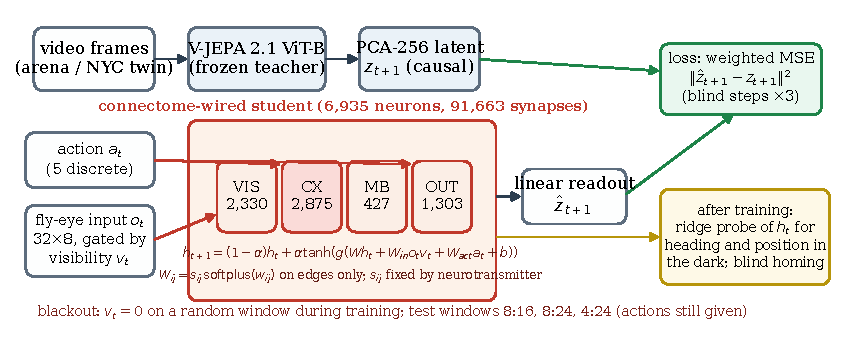
\includegraphics[width=\linewidth]{fig/schematic.pdf}
  \caption{\textbf{A video world model, distilled into a fly's wiring diagram.} A frozen \vjepa encoder turns each frame
  of an episode into a causal latent $z_t$. The student is a leaky rate network whose recurrence $W$ lives only on the
  91,663 signed synapses of the \flywire connectome (VIS, CX, MB and OUT populations); training can scale a synapse but
  never flip its sign or add one. The single training signal is next-latent prediction, with the visual input randomly
  cut (``blackout'') so that the state must carry the latent forward from the action record alone. Everything we
  report about heading, position and homing is read out of the trained state afterwards; none of it was supervised.}
  \label{fig:schematic}
\end{figure*}

Ask a world model to imagine the next second of a video and it will do a reasonable job. Ask it what it imagines after
the lights go out, and the answer depends entirely on what its recurrent core chose to remember. In most video world
models that core is a generic block, a GRU or a transformer layer, sized by compute budget and trained with nothing
but the prediction loss to guide what it keeps~\cite{ha2018world,hafner2023dreamerv3,assran2025vjepa2}. Biology took a
different route to the same problem. A fruit fly in darkness holds its heading and a vector back to where it started
for many seconds, using a few thousand neurons of its central complex, and the complete synapse-level wiring of that
circuit is now public~\cite{seelig2015neural,green2017neural,turnerevans2017angular,dorkenwald2024neuronal,schlegel2024whole}.

This paper puts the two together and asks a plain question: \emph{if a world model's recurrence is forced to be the
fly's wiring diagram, what does the wiring buy?} We distil \vjepa~\cite{assran2025vjepa2}, a self-supervised video
foundation model, into a leaky rate network of 6,935 \flywire neurons whose only recurrent weights sit on the 91,663
signed synapses of the real connectome (\cref{fig:schematic}). The student never sees the teacher's weights, only its
latent through the loss. It is trained on one objective, next-latent prediction under random blackouts of the visual
input, so any structure that appears in its state was not asked for.

\begin{figure*}[t]
  \centering
  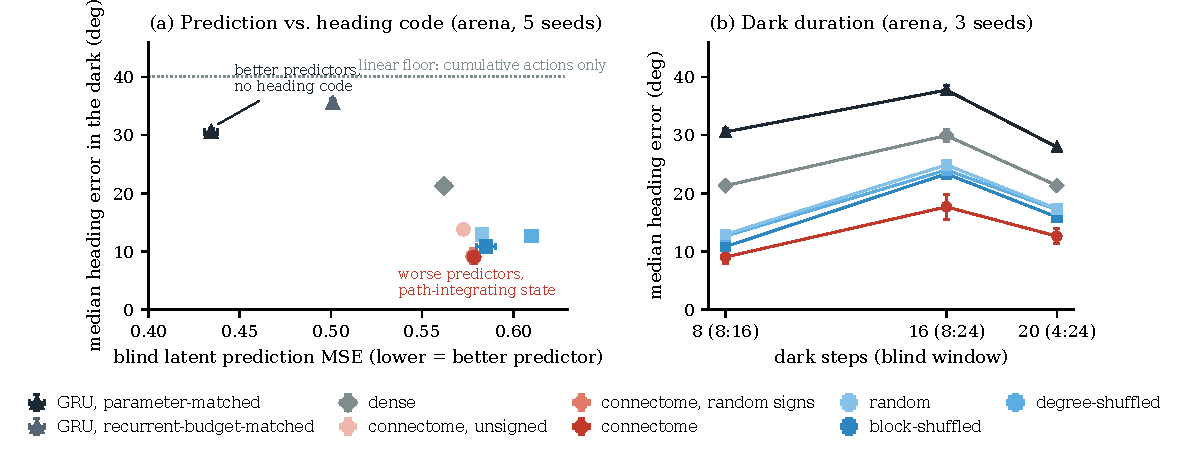
\includegraphics[width=\linewidth]{fig/main_result.pdf}
  \caption{\textbf{The wiring makes a worse predictor and a better integrator.} (a) Each point is one wiring (mean\pm sd
  over 5 seeds): blind latent-prediction error on the $x$-axis, median heading error decoded from the state during 8
  dark steps on the $y$-axis. Both GRUs predict the teacher best and keep almost no heading; the connectome and its
  sparse controls predict worse and keep heading to about 10\degree. A linear readout of the cumulative actions alone
  gives 40\degree\ (dotted). (b) The code degrades gracefully with the length of the dark window, and the real
  wiring's margin over block-shuffled grows from 2\degree\ to 6\degree\ at 16 dark steps.}
  \label{fig:main}
\end{figure*}

The answer has two halves, and we think both are worth stating plainly. The wiring is \emph{not} a better predictor.
Against controls that hold neuron count, edge count, region block structure, Dale's-law sign structure and parameter
count fixed, the real connectome beats its shuffled twins by about one percent of latent error, consistently, while a
parameter-matched GRU is 25\,\% better and a GRU matched to the connectome's \emph{recurrent} budget is still 13\,\%
better. What the wiring buys instead is a \emph{path-integrating state} (\cref{fig:main}). During the blind steps a
ridge probe reads heading from the connectome state to 9\degree\ median error and position to $R^2$\,0.94. The
parameter-matched GRU, which predicts the latent far better, gives 31\degree\ and 0.41; the budget-matched GRU gives
36\degree\ and 0.30; a linear readout of the action history, which is all the state could possibly have integrated,
gives 40\degree. The code survives 16 and 20 dark steps, shows up again in a city-scale raycast twin of Manhattan, and
widens rather than closes under a non-linear probe.

Three further findings keep the claim honest, and we report all of them in full. First, sparse random and
block-shuffled wirings of the same size form the code too, 2\degree\ to 6\degree\ worse than the real graph; the exact
synapse list is a small, reproducible bonus, not the cause. Second, a linear readout of the state drives blind homing
well above a random-action floor (NYC twin: 37\,\% success against 0\,\%) but well below a dead-reckoning ceiling
(92\,\%), and steering toward a decoded goal vector does not beat random actions. The controller is not the bottleneck;
the readout is. Third, on real handheld video no student, fine-tuned or not, beats a copy-last-visible baseline.

\paragraph{Contributions}
\begin{itemize}
  \item A distillation recipe that turns a video foundation model into a world model whose recurrence is a fixed,
        signed, biologically sourced sparse graph, with controls that separate wiring identity from density, degree
        sequence, region structure and sign structure (\cref{sec:method}).
  \item The first demonstration, to our knowledge, that a connectome-wired latent predictor forms a linearly readable
        heading and position code in the dark that a GRU trained on the same objective does not, with the
        information-ceiling, feature-count and non-linearity controls needed to read that result correctly
        (\cref{sec:probes}).
  \item A behavioural test of that code (blind homing, goal-vector navigation) with oracle, dead-reckoning and random
        controls, reported in full including the negative outcomes, plus cost, data efficiency, scaling, subgraph
        ablation and real-video transfer (\cref{sec:behaviour,sec:more}).
  \item Two environments (a 360\degree\ arena and a raycast twin of Midtown Manhattan), the full pipeline, and all 424
        checkpoints across 5 seeds and 12 wirings, released for reuse.
\end{itemize}

\section{Related work}
\label{sec:related}

\paragraph{Vision world models}
Following the taxonomy of Yu \etal~\cite{yu2026seeing}, vision world models fall into four design families: sequential
token generation~\cite{bruce2024genie}, diffusion-based generation~\cite{agarwal2025cosmos,bar2024nwm}, embedding
prediction~\cite{lecun2022path,bardes2024vjepa,assran2025vjepa2,zhou2024dinowm,baldassarre2025dinoworld}, and latent
state transition~\cite{ha2018world,hafner2023dreamerv3,micheli2023iris,zhang2023storm,robine2023twm}. Our student is an
embedding-prediction model with a state-transition core: a frozen \vjepa encoder supplies the target space, as DINO-WM
and DINO-world do with frozen DINO features~\cite{zhou2024dinowm,baldassarre2025dinoworld}, and a recurrent network
carries the latent through time under actions, as the recurrent state-space models of Dreamer~\cite{hafner2023dreamerv3}
and the transformer cores of IRIS, STORM and TWM~\cite{micheli2023iris,zhang2023storm,robine2023twm} do. The field's
recurrent core is a free architectural choice sized by compute; ours is fixed by a wiring diagram. We therefore compare
against the two cores a reviewer would ask for by name, a gated recurrent unit and a causal transformer predictor, both
matched to the student's parameter budget, and against the trivial copy-last and constant predictors every world-model
benchmark reports~\cite{bar2024nwm}. Knowledge distillation~\cite{hinton2015distilling} usually compresses a model into
a smaller member of the same family; here the target is a fixed, signed, biologically sourced sparse graph.

\paragraph{Navigation world models and embodied evaluation}
Navigation World Models~\cite{bar2024nwm} plan trajectories in a diffusion video model and evaluate with the
success-rate and SPL protocol of embodied navigation~\cite{anderson2018evaluation}; DINO-WM plans zero-shot in a frozen
latent space~\cite{zhou2024dinowm}. We adopt the same metrics for blind homing and goal-vector navigation, and the same
distinction between open-loop prediction and closed-loop control, which is where our behavioural results stop short.

\paragraph{Connectome-constrained models}
Whole-brain \emph{Drosophila} connectomes~\cite{dorkenwald2024neuronal,schlegel2024whole} with predicted neurotransmitter
signs~\cite{eckstein2024neurotransmitter} have enabled models whose connectivity is read off the wiring diagram rather than
learned. Lappalainen \etal~\cite{lappalainen2024connectome} fit a connectome-constrained visual system to a motion task
and predicted neural recordings; models of the central complex~\cite{hulse2021connectome,stone2017anatomically}
explain heading and path-integration circuits mechanistically. These works fit neural data or hand-designed tasks. We
instead distil a self-supervised video model into the wiring and measure what the wiring does to a world model,
with matched-control analysis as the main instrument.

\paragraph{Path integration in artificial networks}
Recurrent networks trained to localise from velocity input develop grid- and head-direction-like
codes~\cite{cueva2018emergence,banino2018vector,sorscher2019unified}. In those studies the task \emph{is} localisation.
Here the task is latent video prediction; heading and position are never supervised, and the probe results show that
whether such a code forms depends on the recurrent topology, not only on the objective.

\paragraph{Controls for wiring identity}
Degree-preserving rewiring~\cite{maslov2002specificity} is the standard null model for network structure. We extend it
with a block-preserving variant that keeps within-region degree sequences and the region-to-region edge counts, so that
the comparison isolates synapse-level identity from the macro-architecture, and with sign controls that keep Dale's law
while randomising which neuron is excitatory.

\section{Method}
\label{sec:method}

\subsection{Environments and episodes}
\label{sec:envs}

\begin{figure}[t]
  \centering
  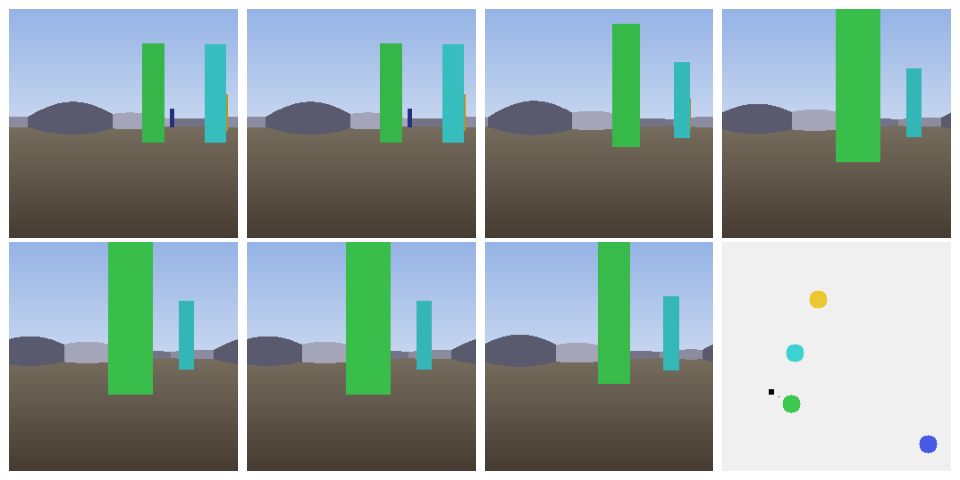
\includegraphics[width=0.49\linewidth]{fig/env_nav.png}\hfill
  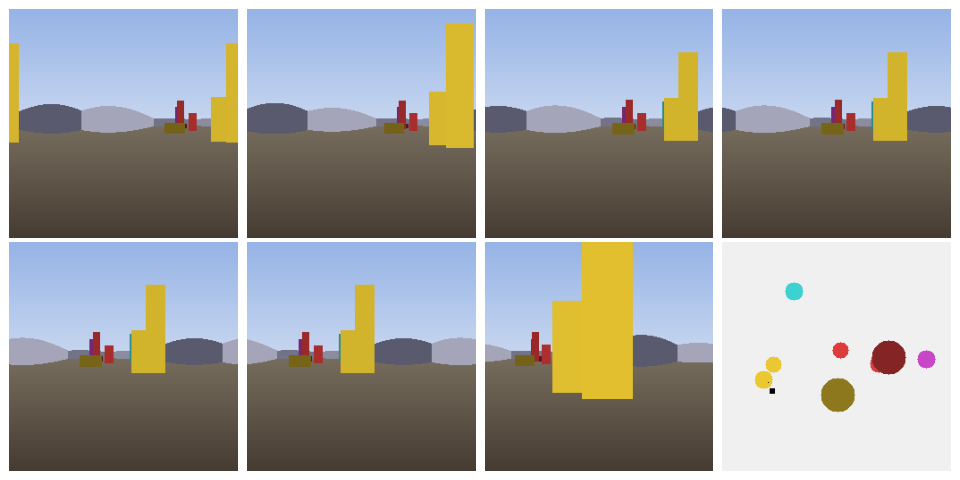
\includegraphics[width=0.49\linewidth]{fig/env_arrange.png}\\[2pt]
  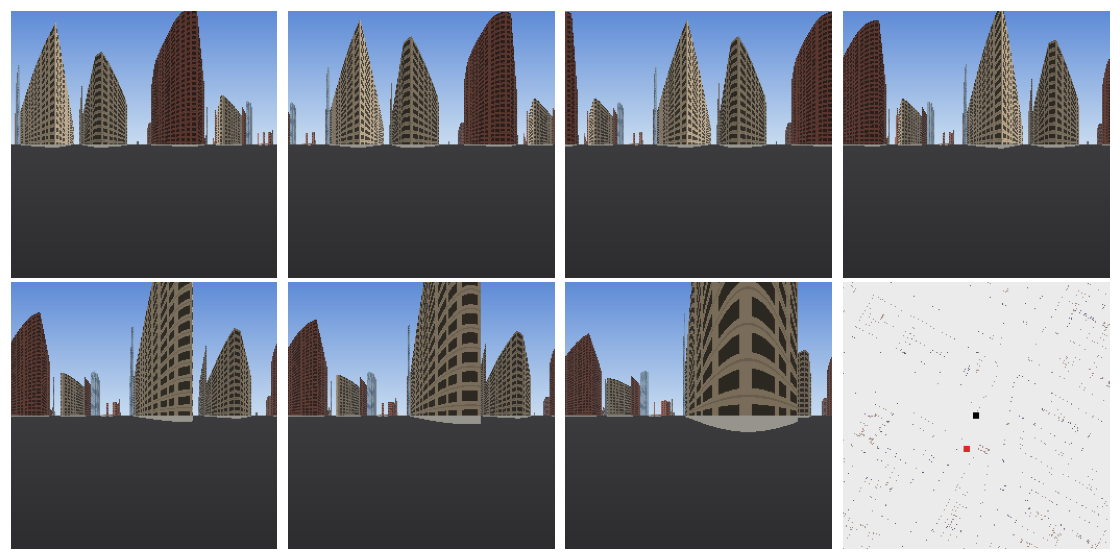
\includegraphics[width=\linewidth]{fig/env_nyc.png}
  \caption{\textbf{Environments.} Top: the 360\degree\ arena as the teacher sees it, for the \textsc{nav} (left) and
  \textsc{arrange} (right) tasks. Bottom: seven steps of one episode in the raycast twin of Midtown Manhattan and its
  top-down map (start in black, goal in red).}
  \label{fig:envs}
\end{figure}

\paragraph{Arena} A 360\degree\ cylindrical panorama rendered at 256\,px with coloured blocks on a ground plane
(\cref{fig:envs}, top). Two tasks share the action space: \textsc{nav} (reach a target block) and \textsc{arrange}
(push blocks to a layout). Five discrete actions: stay, forward 0.6 units, turn left or right 22.5\degree, back 0.36.
Episodes are 24 steps under a scripted policy; 1,000 training and 200 test episodes.

\paragraph{NYC twin} A raycast model of Midtown Manhattan built from building footprints (\cref{fig:envs}, bottom):
forward-facing 110\degree\ camera at 256\,px, forward 4\,m, back 2\,m, goals 30 to 60\,m away; 120 training and 30
test episodes at Times Square, 3 seeds. It adds occlusion, perspective and a real street graph to the arena's clean
geometry.

\paragraph{Blackouts} During training, each episode has a random contiguous window in which the visual input is
replaced by zero and only the action is given. At test the window is steps 8 to 16 unless stated (also 8 to 24 and 4 to
24). The student's job in the window is to carry the teacher's latent forward from the action record.

\subsection{Teacher}
The teacher is \vjepa ViT-B~\cite{assran2025vjepa2} applied to 16-frame clips (each environment step duplicated into one
tubelet). Per-step targets are the mean token concatenated with $2\times2$ pooled tokens (3,840-d), projected to a
PCA-256 basis fit on the training set (94.6\,\% of the variance on the arena, 91.0\,\% on NYC) and whitened by one
scalar. Targets are \emph{causal}: the clip for step $t$ ends at $t$, so a blind target never contains frames the student
has not seen. All MSE values are in this whitened PCA space; the teacher-space equivalents are in the supplement.

\subsection{Connectome subgraph}
\label{sec:connectome}
From \flywire v783~\cite{dorkenwald2024neuronal,schlegel2024whole} we take 6,935 neurons in four populations: VIS
(2,330; TuBu, MeTu, LC and LPLC visual projection neurons that feed the central complex and optic glomeruli), CX (2,875;
all central-complex cell classes, including EPG, PEN, $\Delta$7, PFN, PFL, h$\Delta$, FC, ER and ExR), MB (427; mushroom-body
output and dopaminergic neurons) and OUT (1,303; descending neurons). Edges are the 91,663 directed pairs with at least
5 synapses. The sign of every edge is the sign of its presynaptic neuron's predicted
neurotransmitter~\cite{eckstein2024neurotransmitter} (ACh, DA, 5-HT, OA excitatory; Glu, GABA inhibitory; 49.9\,\%
excitatory), so Dale's law holds by construction. The subgraph is a central-complex-centred navigation circuit, not a
whole-brain model; \cref{sec:ablation} ablates the synapse threshold and the region choice.

\subsection{Student}
\label{sec:student}
The student is a leaky tanh rate network on the connectome's neurons,
\begin{equation}
  h_{t+1} = (1-\alpha)\,h_t + \alpha\tanh\!\big(g\,(W h_t + W_{\text{in}}\, o_t \cdot v_t + W_{\text{act}}\, a_t + b)\big),
  \label{eq:student}
\end{equation}
with $\alpha = 0.5$, gain $g$, visual input $o_t$ (a $32\times8\times3$ fly-eye downsample of the panorama) gated by the
visibility flag $v_t$, and the one-hot action $a_t$. $W$ is non-zero only on connectome edges and is parametrised as
$W_{ij} = s_{ij}\,\mathrm{softplus}(w_{ij})$ with $s_{ij}$ the fixed sign, so training can change synaptic strength but
never sign or existence. Visual input enters VIS neurons only; the action enters CX and OUT neurons; a linear readout
from all neurons predicts the teacher latent. The recurrence has 91,663 parameters; $W_{\text{in}}$ (VIS rows only) and
the readout add 3.6\,M, identical for every sparse wiring. One step costs $O(E)$ on the edge list.

\paragraph{Loss} Weighted MSE to the whitened teacher latent at every step, blind steps weighted $3\times$, plus
$10^{-4}\,\overline{h^2}$. There is no feature-alignment or policy term; nothing about heading, position or actions is
supervised.

\subsection{Controls}
\label{sec:controls}
All sparse controls keep the neuron set, the region labels, the input and output routing, the exact edge count, the
absence of self-loops, and Dale-consistent signs at the real excitatory fraction.
\begin{itemize}
  \item \textbf{block-shuffled}: Maslov--Sneppen rewiring~\cite{maslov2002specificity} within each region-to-region
        block, preserving every neuron's in- and out-degree per block and all block edge counts. This is the key
        control: it keeps the macro-architecture and destroys only synapse identity.
  \item \textbf{degree-shuffled}: global Maslov--Sneppen rewiring, preserving degrees but not blocks.
  \item \textbf{random}: Erd\H{o}s--R\'enyi with the same edge count.
  \item \textbf{random signs}: the real graph with neuron signs permuted (Dale's law kept, which neuron is
        excitatory randomised). \textbf{unsigned}: the real graph with free-sign weights.
  \item \textbf{dense}: all $6{,}935^2$ recurrent weights free (51.7\,M parameters).
  \item \textbf{GRU}: a gated recurrent unit~\cite{cho2014learning} with 762 hidden units, matched to the sparse student's
        \emph{total} parameter count (3.71\,M), receiving the same input, action and visibility flag.
  \item \textbf{GRU, recurrent-budget-matched}: 174 hidden units, 90,828 recurrent weights, matched to the connectome's
        \emph{recurrent} parameter count (0.54\,M in total).
\end{itemize}
Learning rates were selected per architecture on a validation split. Five seeds on the arena, three on NYC. Paired
comparisons use the shared test episodes; we report mean\pm sd over seeds and 95\,\% $t$-intervals where $n \ge 3$.

\subsection{Probes and behavioural readouts}
\label{sec:probe-method}
\paragraph{Probes} Ridge regression from the state $h_t$ to heading (as $\sin,\cos$) and position relative to the
start of the blind window, fit on training episodes, evaluated on test episodes inside the window. We report the median
absolute heading error and position $R^2$. An MLP probe (one hidden layer, 256 units) tests whether a code is present
but non-linear. Two reference rows are essential: \emph{actions only}, the same probe on the cumulative one-hot action
history (what any integrator of the action input exposes), and \emph{integrator}, closed-form dead reckoning of the
action record, which is exact for heading because turns are fixed-angle. Feature-count controls use random neuron
subsets of the GRU's width.

\paragraph{Blind homing} The agent walks out under the scripted policy for 12 visible steps; vision is then cut and a
controller steers for 24 steps from a pose estimate. Success is ending within 1 arena unit (12\,m on NYC) of the start.
The pose estimate comes from a ridge readout of the state, fit on training episodes plus 300 closed-loop rollouts in
fresh arenas; the same controller is run with the \emph{oracle} pose, with \emph{dead reckoning} of the action record,
and with \emph{random} actions.

\paragraph{Goal-vector navigation} The same controller steers toward a linearly decoded egocentric goal vector for 40
steps, with and without a 3- or 5-step vision cut, against the true goal vector and random actions.

\section{Experiments}
\label{sec:experiments}

Every number in this section is produced by \texttt{scripts/make\_paper\_tables.py} from the released result files;
the tables are included verbatim. Arena and continuous-turn results are over \nSeeds\ seeds, NYC over \nSeedsNyc.

\subsection{Prediction accuracy is not what the wiring buys}
\label{sec:prediction}

\begin{table*}[t]
  \centering\small
  \setlength{\tabcolsep}{4pt}
  \begin{tabular}{lcccccc}
    \toprule
    & \multicolumn{2}{c}{Arena (5 seeds)} & \multicolumn{2}{c}{Cont.\ turns (0 seeds)} & \multicolumn{2}{c}{NYC twin (3 seeds)} \\
    \cmidrule(lr){2-3}\cmidrule(lr){4-5}\cmidrule(lr){6-7}
    wiring & MSE $\downarrow$ & cos $\uparrow$ & MSE $\downarrow$ & cos $\uparrow$ & MSE $\downarrow$ & cos $\uparrow$ \\
    \midrule
    GRU, parameter-matched & \textbf{0.434\pm0.004} & \textbf{0.72} & -- & -- & \textbf{0.609\pm0.003} & \textbf{0.56} \\
    GRU, recurrent-budget-matched & 0.501\pm0.001 & 0.67 & -- & -- & -- & -- \\
    dense & 0.562\pm0.004 & 0.63 & -- & -- & -- & -- \\
    connectome, unsigned & 0.573\pm0.001 & 0.63 & -- & -- & -- & -- \\
    connectome, random signs & 0.578\pm0.001 & 0.62 & -- & -- & -- & -- \\
    \textbf{connectome} & 0.579\pm0.003 & 0.62 & -- & -- & 0.701\pm0.010 & 0.47 \\
    random & 0.583\pm0.002 & 0.61 & -- & -- & 0.707\pm0.007 & 0.48 \\
    block-shuffled & 0.585\pm0.005 & 0.61 & -- & -- & 0.726\pm0.014 & 0.45 \\
    degree-shuffled & 0.610\pm0.002 & 0.59 & -- & -- & 0.731\pm0.005 & 0.45 \\
    \midrule
    copy last visible latent & 0.811 & -- & -- & -- & 1.558 & -- \\
    constant mean & 0.992 & -- & -- & -- & 0.977 & -- \\
    \bottomrule
\end{tabular}

  \caption{\textbf{Blind-horizon latent prediction.} Mean MSE over blind horizons 1 to 8 in whitened PCA-256 space
  (mean\pm sd over seeds) and cosine to the teacher latent, on the arena, on the arena with continuous turn angles and
  on the NYC twin. Every student beats both trivial predictors. The parameter-matched GRU and transformer beat every
  sparse student; among sparse wirings of identical size the real connectome is the best by about one percent. The
  attention-input rows replace the shared linear input map by a per-neuron cross-attention encoder (\cref{sec:student});
  the hybrid row adds one attention layer over cell-type tokens to the connectome recurrence.}
  \label{tab:pred}
\end{table*}

\cref{tab:pred} gives the headline prediction numbers. Every student is far below both trivial predictors. Among sparse
wirings of identical size the real connectome is the best, by \nConnOverBlockArena\,\% of latent error over
block-shuffled, and the margin is reproducible: it holds on every seed, on the continuous-turn data, on the NYC twin, at
every training-set size from 50 to 500 episodes (\cref{sec:suppl-data}) and on every subgraph we ablate
(\cref{sec:ablation}). But it is small, and the dense sequence models are clearly better: the parameter-matched GRU by
\nGruBetterArena\,\%, the parameter-matched transformer by \nTfBetterArena\,\% (\nGruBetterNyc\ and \nTfBetterNyc\,\% on
NYC). Sign structure does not help prediction either: the unsigned student is marginally better than the signed one.
We therefore make no claim that the connectome is a better predictor. It is a worse one, and what follows is about what
it does instead.

\subsection{The connectome state path-integrates in the dark}
\label{sec:probes}

\begin{table*}[t]
  \centering\small
  \setlength{\tabcolsep}{3.5pt}
  \begin{tabular}{lcccccc}
    \toprule
    & \multicolumn{2}{c}{Arena} & \multicolumn{2}{c}{Continuous turns} & \multicolumn{2}{c}{NYC twin} \\
    \cmidrule(lr){2-3}\cmidrule(lr){4-5}\cmidrule(lr){6-7}
    wiring & heading err & pos $R^2$ & heading err & pos $R^2$ & heading err & pos $R^2$ \\
    \midrule
    GRU, parameter-matched & 30.6\pm0.6 & 0.41\pm0.01 & -- & -- & 45.4\pm2.6 & 0.25\pm0.01 \\
    GRU, recurrent-budget-matched & 35.5\pm0.7 & 0.30\pm0.01 & -- & -- & -- & -- \\
    dense & 21.3\pm0.7 & 0.68\pm0.01 & -- & -- & -- & -- \\
    connectome, unsigned & 13.8\pm0.8 & 0.88\pm0.01 & -- & -- & -- & -- \\
    connectome, random signs & 9.2\pm1.3 & \textbf{0.94\pm0.01} & -- & -- & -- & -- \\
    \textbf{connectome} & \textbf{9.1\pm1.2} & 0.94\pm0.01 & -- & -- & \textbf{9.4\pm0.7} & \textbf{0.94\pm0.01} \\
    random & 12.9\pm0.7 & 0.88\pm0.01 & -- & -- & 15.1\pm0.7 & 0.89\pm0.00 \\
    block-shuffled & 10.8\pm0.8 & 0.93\pm0.01 & -- & -- & 10.1\pm1.1 & 0.94\pm0.02 \\
    degree-shuffled & 12.7\pm0.6 & 0.89\pm0.02 & -- & -- & 14.3\pm2.0 & 0.84\pm0.01 \\
    \midrule
    actions only (linear floor) & 40.1 & 0.54 & -- & -- & 22.6 & 0.41 \\
    integrator of the action record & 0.0 & 1.00 & -- & -- & 0.0 & 1.00 \\
    \bottomrule
\end{tabular}

  \caption{\textbf{Heading and position decoded from the state during 8 blind steps.} Ridge probe; median absolute
  heading error in degrees and position $R^2$ relative to the start of the window, mean\pm sd over seeds. With
  continuous turn angles the action record no longer determines heading, so the integrator row is no longer exact and
  the probe measures integration of a noisy signal. The connectome keeps a linearly readable heading and position code
  that neither the GRU nor the transformer forms; sparse controls of the same size form a slightly worse one.}
  \label{tab:probe}
\end{table*}

\cref{tab:probe} and \cref{fig:main} are the main result. During the 8 blind steps the connectome state carries heading
to \nConnArenaHd\degree\ median error and position to $R^2$\,\nConnArenaPos\ on the arena, \nConnNycHd\degree\ and
\nConnNycPos\ on NYC. The parameter-matched GRU, which predicts the teacher far better, gives \nGruArenaHd\degree\ and
\nGruArenaPos\ on the arena; the transformer, which also predicts better and can attend over its whole visible past,
gives \nTfArenaHd\degree\ and \nTfArenaPos. Three controls fix what this does and does not mean.

\paragraph{Information ceiling} With fixed-angle turns and actions given in the dark, a closed-form integrator of the
action record recovers heading exactly, so on the arena the probe does not ask whether heading \emph{can} be known; it
asks whether the state \emph{keeps} it in a population code a linear readout can use. A linear probe on the cumulative
action counts alone reaches \nActOnlyArenaHd\degree\ (a linearity floor, not an information floor). The continuous-turn
columns remove the ceiling: every turn is scaled by a $\mathcal{N}(1, 0.3)$ factor, the integrator of the discrete record
is wrong by \nIntegratorTnHd\degree\ on median, and the connectome state decodes to \nConnTnHd\degree. Whatever it
integrates there is not the action record.

\paragraph{Non-linearity} \cref{tab:dark} repeats the probe with an MLP. An MLP on the GRU state gives
\nGruArenaMlpHd\degree, so the GRU is not hiding the code non-linearly; on the sparse students the same probe
\emph{improves} heading to \nConnArenaMlpHd\degree\ (connectome) and \nBlockArenaMlpHd\degree\ (block-shuffled). The
gap widens under the non-linear probe.

\paragraph{Feature count} A random 762-neuron subset of the connectome (the GRU's width) decodes heading at
19\degree, still better than the full GRU state (\cref{sec:suppl-probe}).

\paragraph{What the wiring contributes} Sign structure matters, but not which signs: the unsigned student loses the
code (\nNosignArenaHd\degree, $R^2$\,\nNosignArenaPos) while random Dale-consistent signs match the real ones. The exact
synapse list matters a little: the real wiring beats block-shuffled by \nConnBlockGapArena\degree\ on the arena and
\nConnBlockGapNyc\degree\ on NYC, consistently across seeds.

\paragraph{Not region-specific} The 51 EPG neurons that form the biological heading ring carry almost no heading
(50\degree), and the central complex as a whole (12.6\degree) decodes no better than a random subset of the same size
(10.7\degree). We make no ring-attractor claim.

\begin{table*}[t]
  \centering\small
  \setlength{\tabcolsep}{5pt}
  \begin{tabular}{lcccc}
    \toprule
    wiring & ridge, 8 dark (8:16) & MLP, 8 dark & ridge, 16 dark (8:24) & ridge, 20 dark (4:24) \\
    \midrule
    GRU, parameter-matched & 30.6\pm0.6, 0.41 & 27.4\pm0.3, 0.42 & 37.7\pm0.8, 0.32 & 27.9\pm0.3, 0.50 \\
    GRU, recurrent-budget-matched & 35.5\pm0.7, 0.30 & 32.4\pm0.4, 0.32 & 44.8\pm0.5, 0.21 & 33.7\pm1.0, 0.35 \\
    dense & 21.3\pm0.7, 0.68 & 41.2\pm24.2, 0.27 & 29.9\pm1.1, 0.46 & 21.3\pm0.5, 0.53 \\
    connectome, unsigned & 13.8\pm0.8, 0.88 & -- & -- & -- \\
    connectome, random signs & 9.2\pm1.3, 0.94 & \textbf{4.7\pm0.3, 0.89} & 18.6\pm1.1, 0.82 & 13.6\pm1.4, 0.82 \\
    \textbf{connectome} & \textbf{9.1\pm1.2, 0.94} & 4.7\pm0.1, 0.87 & \textbf{17.7\pm2.1, 0.82} & \textbf{12.6\pm1.2, 0.82} \\
    random & 12.9\pm0.7, 0.88 & 6.4\pm0.4, 0.83 & 24.9\pm0.6, 0.72 & 17.3\pm0.6, 0.77 \\
    block-shuffled & 10.8\pm0.8, 0.93 & 5.9\pm0.3, 0.86 & 23.3\pm0.4, 0.77 & 15.9\pm0.6, 0.77 \\
    degree-shuffled & 12.7\pm0.6, 0.89 & 6.9\pm0.7, 0.83 & 24.0\pm1.0, 0.71 & 17.2\pm0.6, 0.76 \\
    \bottomrule
\end{tabular}

  \caption{\textbf{Probe type and dark duration, arena.} Median heading error (\degree) and position $R^2$ under a
  ridge and an MLP probe over 8 dark steps, and under the ridge probe over 16 and 20 dark steps. The real wiring's
  margin over block-shuffled grows from \nConnBlockGapArena\degree\ to \nConnBlockGapArenaDarkSixteen\degree\ at 16 dark steps.}
  \label{tab:dark}
\end{table*}

\begin{figure*}[t]
  \centering
  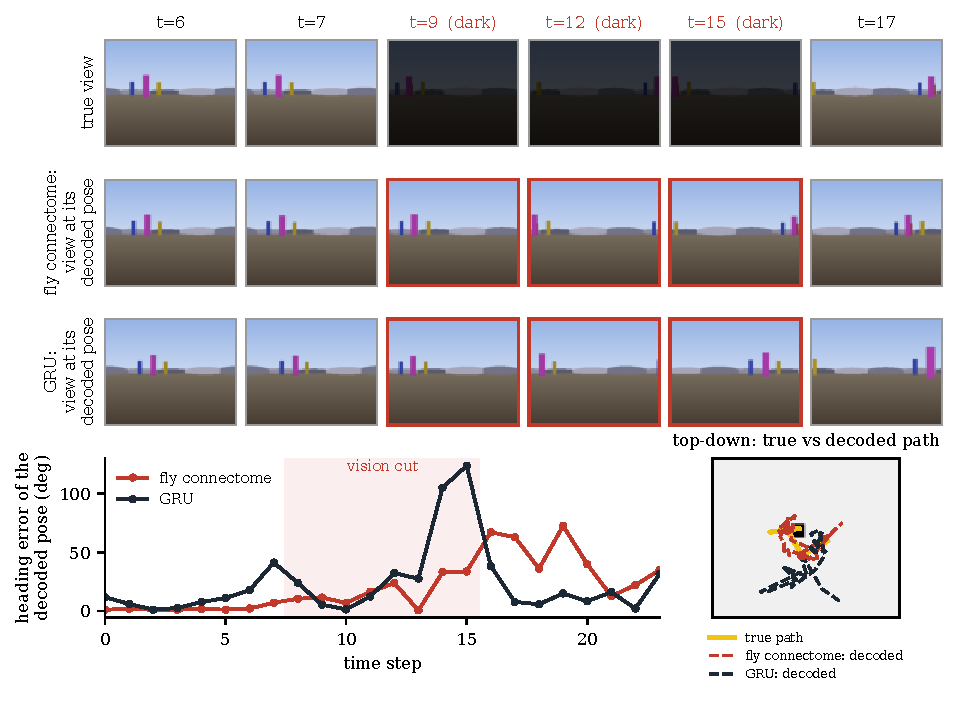
\includegraphics[width=\linewidth]{fig/video_strip.pdf}
  \caption{\textbf{What each network sees, thinks and decodes through a blackout} (one test episode, chosen as the one
  closest to the population medians for both models; video in the supplement). Top row: the panorama the teacher
  receives, dimmed during the vision cut. Middle rows: the arena rendered at the pose that a ridge readout decodes from
  each student's own activity at that moment, so each frame is literally where the network thinks it is. The connectome
  student's decoded view stays locked to the true view through the dark; the GRU's drifts. Bottom: heading error of the
  decoded pose over time, and the true path against both decoded paths. Both readouts show a transient when vision
  returns at $t{=}16$. The readout is fit on 400 training episodes and never sees this episode.}
  \label{fig:strip}
\end{figure*}

\paragraph{Seeing it} \cref{fig:strip} shows the effect on one episode: with vision cut, the pose read out of the
connectome state keeps rendering the right view, while the pose read out of the GRU state wanders. The interactive
version of this figure, with the live neuron state on the FlyWire coordinates, is in the supplement.

\paragraph{Dark duration} \cref{tab:dark} lengthens the window. Over 16 dark steps the connectome keeps heading
within \nConnArenaDarkSixteenHd\degree\ where the GRU is at \nGruArenaDarkSixteenHd\degree, and the real wiring's margin over
block-shuffled grows from \nConnBlockGapArena\degree\ to \nConnBlockGapArenaDarkSixteen\degree.

\subsection{Where the gap between sparse and dense models lives}
\label{sec:gap}

The attention-input rows of \cref{tab:pred,tab:probe} remove the one component the sparse students share with no
biological circuit: the 1.8\,M-parameter linear map from the fly-eye image into the VIS neurons. With a per-neuron
cross-attention encoder of 0.11\,M parameters, and the GRU and transformer re-matched to the smaller budget, the
sparse students predict at \nConnAttnArenaMse\ against \nGruAttnArenaMse\ (GRU) and \nTfAttnArenaMse\ (transformer),
and decode heading at \nConnAttnArenaHd\degree\ against \nGruAttnArenaHd\ and \nTfAttnArenaHd\degree. The prediction gap
therefore does not come from the input map, and the path-integration gap survives a better one.

The hybrid row asks the converse: what does the connectome lack? Adding one self-attention layer over the 796
cell-type-pooled activities to the recurrence (30\,k parameters, edge list unchanged) moves prediction to
\nHybridArenaMse\ and heading to \nHybridArenaHd\degree. \TODO{interpret once run 2 lands: does global routing close the
prediction gap, and does the code survive it?}

\subsection{Behaviour from the code}
\label{sec:behaviour}

\begin{figure*}[t]
  \centering
  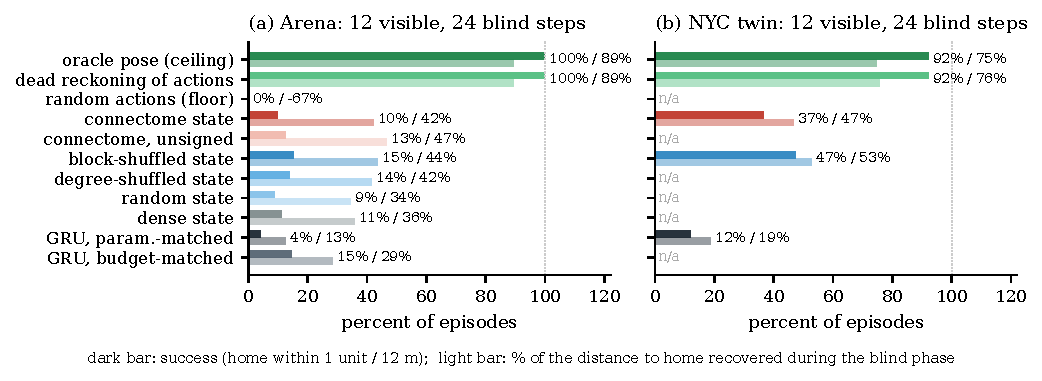
\includegraphics[width=\linewidth]{fig/homing.pdf}
  \caption{\textbf{Blind homing.} After 12 visible steps vision is cut and the same controller steers for 24 steps from
  one of several pose estimates. With the true pose or with dead reckoning of the action record it gets home almost
  every time, so the controller is not the limit. From a linear readout of a connectome-sized sparse state the agent
  recovers about half the distance; from the GRU or transformer state it barely moves. The real wiring has no edge over
  block-shuffled here.}
  \label{fig:homing}
\end{figure*}

\begin{table*}[t]
  \centering\small
  \setlength{\tabcolsep}{3.5pt}
  \begin{tabular}{lcccccc}
    \toprule
    & \multicolumn{2}{c}{Arena} & \multicolumn{2}{c}{Continuous turns} & \multicolumn{2}{c}{NYC twin} \\
    \cmidrule(lr){2-3}\cmidrule(lr){4-5}\cmidrule(lr){6-7}
    pose readout & \% closer & success & \% closer & success & \% closer & success \\
    \midrule
    oracle pose (controller ceiling) & 89 & 1.00 & -- & -- & 75 & 0.92 \\
    dead reckoning of actions & 89 & 1.00 & 87 & 0.90 & 76 & 0.92 \\
    random actions (floor) & -67 & 0.00 & -- & -- & -- & -- \\
    \midrule
    GRU, parameter-matched state & 13 & 0.04 & 21 & 0.16 & 19 & 0.12 \\
    GRU, recurrent-budget-matched state & 29 & 0.15 & -- & -- & -- & -- \\
    dense state & 36 & 0.11 & -- & -- & -- & -- \\
    connectome, unsigned state & \textbf{47} & 0.13 & -- & -- & -- & -- \\
    \textbf{connectome} state & 42 & 0.10 & \textbf{33} & \textbf{0.16} & 47 & 0.37 \\
    random state & 34 & 0.09 & -- & -- & -- & -- \\
    block-shuffled state & 44 & \textbf{0.15} & -- & -- & \textbf{53} & \textbf{0.47} \\
    degree-shuffled state & 42 & 0.14 & -- & -- & -- & -- \\
    \bottomrule
\end{tabular}

  \caption{\textbf{Blind homing from a linear readout of the state.} 12 visible then 24 blind steps; 50 test episodes
  per seed. \% closer is the reduction of the distance to home over the blind phase. On the continuous-turn arena the
  dead-reckoning controller is itself noisy. Every connectome-sized sparse student halves its distance from a linear
  readout; the GRU and transformer barely move. The real wiring has no edge over block-shuffled here.}
  \label{tab:homing}
\end{table*}

\cref{fig:homing} and \cref{tab:homing} ask whether the code is usable. The controller is not the bottleneck: with the
oracle pose or with dead reckoning of the action record it reaches home in almost every episode. From a linear readout
of the connectome state the agent recovers \nConnArenaCloser\,\% of its distance to home on the arena and
\nConnNycCloser\,\% on NYC, reaching it in \nConnNycSucc\ of NYC episodes, against \nGruNycSucc\ for the GRU and
\nTfNycSucc\ for the transformer. But arena success is only \nConnArenaSucc, and on NYC block-shuffled wiring does as
well or better. The behavioural effect is carried by connectome-scale sparse recurrence, not by synapse identity, and
the gap to the ceiling is the drift of a linear pose readout over 24 dark steps.

\paragraph{Goal-vector navigation (negative)} Steering toward a linearly decoded egocentric goal vector succeeds in
22\,\% of arena episodes for every wiring (GRU 22, random 21, dense 20) against 14\,\% for random actions and
92\,\% for the true goal vector; 5\,\% on NYC against 0 and 28. A 3- or 5-step vision cut changes nothing. The decoded
goal vector ($R^2$\,0.42 on closed-loop rollouts) is too coarse to steer with, and no wiring is better than another
(\cref{sec:suppl-goalnav}).

\subsection{Real handheld video}
\label{sec:realvid}

\begin{table*}[t]
  \centering\small
  \setlength{\tabcolsep}{4pt}
  \begin{tabular}{lcccccc}
    \toprule
    wiring & zero-shot MSE & fine-tuned MSE & heading, sim.\ readout & heading, clip readout & NYC model, zero-shot & NYC model, fine-tuned \\
    \midrule
    GRU, parameter-matched & 9.94\pm0.07 & \textbf{1.18\pm0.00} & 84.1\pm34.2 & 7.6\pm0.7 & \textbf{5.57\pm0.03} & -- \\
    dense & 9.73\pm0.07 & 1.21\pm0.04 & 29.5\pm6.4 & 9.1\pm0.9 & -- & -- \\
    connectome, unsigned & 9.59\pm0.13 & 1.26\pm0.00 & \textbf{24.3\pm6.3} & 7.7\pm0.3 & -- & -- \\
    \textbf{connectome} & 9.68\pm0.10 & 1.24\pm0.02 & 30.9\pm22.8 & 7.7\pm0.5 & 6.10\pm0.03 & -- \\
    random & \textbf{9.56\pm0.19} & 1.26\pm0.01 & 79.1\pm14.5 & 9.9\pm1.1 & 6.00\pm0.02 & -- \\
    degree-shuffled & 9.69\pm0.09 & 1.25\pm0.02 & 88.7\pm27.0 & \textbf{7.1\pm0.6} & 6.01\pm0.05 & -- \\
    \midrule
    copy last visible latent & 0.84 & 0.84 & -- & -- & 0.84 & 0.84 \\
    constant mean & 10.28 & 10.28 & -- & -- & 10.28 & 10.28 \\
    actions only (linear floor) & -- & -- & -- & 4.7 & -- & -- \\
    \bottomrule
\end{tabular}

  \caption{\textbf{Real phone video as the world.} \nRvClips\ clips, \nRvEpisodes\ episodes, blind window 8:16. Left:
  blind MSE of every arena-trained student zero-shot and after leave-one-clip-out fine-tuning (10 epochs), against the
  trivial predictors on the same episodes. Middle: median heading error of a ridge readout that was fit in the
  simulator and applied to the real state (transfer), and of one fit on the other clips (in-domain), against a linear
  readout of the estimated action record. Right: the same for the students trained on the NYC twin.}
  \label{tab:realvid}
\end{table*}

\begin{figure*}[t]
  \centering
  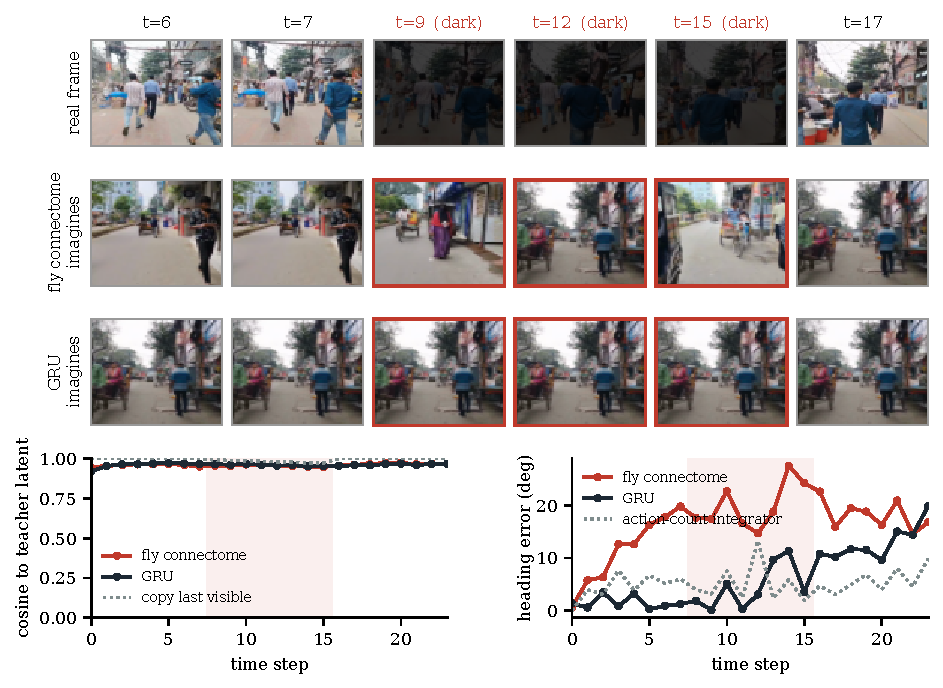
\includegraphics[width=\linewidth]{fig/realvid_strip.pdf}
  \caption{\textbf{The same test on real handheld video} (one held-out phone clip; both students fine-tuned on the
  other clips; video in the supplement). Top: the real frame, dimmed during the vision cut. Middle rows: the training
  frame whose teacher latent is nearest to each student's guess, \ie what each imagines. Bottom left: cosine to the
  teacher latent against a copy-last baseline (dotted). Bottom right: heading decoded from the state against the clip's
  own egomotion estimate, with a plain count of the estimated turn actions (dotted).}
  \label{fig:realvid}
\end{figure*}

\cref{tab:realvid} puts every architecture on the \nRvClips\ phone clips. Zero-shot every student is off distribution
(MSE \nConnRvMse\ for the connectome, \nGruRvMse\ for the GRU, against \nCopyLastRvMse\ for copy-last), and after
fine-tuning all reach about \nConnRvFtMse\ to \nGruRvFtMse, still above the copy-last baseline, because at 2\,Hz the
teacher latent of handheld footage changes little between steps. The heading probe is the informative part. With the
readout fit in the simulator and applied to the real state the connectome decodes the clip's egomotion to
\nConnRvTransferHd\degree\ against \nGruRvTransferHd\degree\ for the GRU; with a readout fit on the other clips the
numbers are \nConnRvIndomainHd\ and \nGruRvIndomainHd\degree\ against \nActOnlyRvHd\degree\ for a linear readout of the
estimated action record. \TODO{state the verdict once run 2 lands: does the simulator-fit heading code transfer to real
footage for the sparse students and not for the dense ones, as in the pilot, and is the in-domain probe above the
action-count floor?} Real video remains the weakest link of the paper: the footage has no odometry ground truth, the
egomotion estimate is itself a model, and the clips are short. We report it in full rather than drop it.

\subsection{Cost, data efficiency, scaling, ablation}
\label{sec:more}

\paragraph{Cost} At batch 1 one connectome step costs 7.4\,MFLOP, the same as the parameter-matched GRU, with 91,663
recurrent weights against the GRU's 580,644; the transformer costs more per step and grows with the context it
attends over; dense costs 103\,MFLOP. The sparse student is cheap in weights, not in wall-clock at this scale, where
every model is launch-bound.

\paragraph{Data efficiency} At 50, 100, 200 and 500 training episodes the ordering of \cref{tab:pred} is unchanged:
the GRU leads at every size and the connectome beats block-shuffled by 1 to 3\,\% (\cref{sec:suppl-data}). A prior
that should matter most with little data does not change the ranking.

\paragraph{Multi-brain scaling} Coupling $K=2$ or $3$ copies of the connectome through the real commissural edges gives
no gain (MSE 0.576, 0.577 vs 0.575 for $K=1$); the heading code is unchanged (7.0\degree, 8.7\degree\ vs 8.5\degree).

\paragraph{Subgraph ablation}
\label{sec:ablation}
With the synapse threshold at 1, 5 or 10, with the mushroom bodies or the descending neurons removed, or with the
central complex alone, the real wiring beats its degree-shuffled twin by 0.02 to 0.04 MSE (one seed each;
\cref{tab:ablation}). No single region carries the margin.

\section{Discussion}
\label{sec:discussion}

\paragraph{Two things that are easy to conflate}
Our experiments pull apart two claims that usually travel together. The first is about a \emph{class} of topology.
Connectome-scale sparse signed recurrence, trained only to predict a video model's latent, ends up holding a state
that path-integrates: heading and position are linearly readable through 8 to 20 dark steps, and a GRU trained on the
same objective, at either parameter budget, never forms this code, even when we look for it with a non-linear probe.
We find this strong, because the GRU predicts the latent better. The code is not a by-product of prediction quality;
if anything it trades against it. The second claim is about the \emph{identity} of the real synapses, and here the
evidence is modest: about one percent of latent error, 2\degree\ to 6\degree\ of heading, reproducible across seeds,
environments, data sizes and subgraphs, but never the cause of the effect and absent from the behavioural readouts.
A reader who takes away only ``sparse signed recurrence integrates, and the fly's version is a little better'' has
understood the paper.

\paragraph{Why might sparse recurrence integrate?}
We can offer a hypothesis but not yet a proof. A sparse signed graph at this scale has a large reservoir of slow,
weakly coupled modes. The leaky update in \cref{eq:student} drives those modes with the action input, and the linear
readout is free to leave them alone because they cost almost nothing in latent error. A gated unit with a dense
$174^2$ or $762^2$ recurrence is pushed by the same objective to spend its capacity on prediction, and nothing in the
loss rewards it for keeping an integral around. The probes on random and shuffled sparse graphs fit this picture: the
code appears whenever the recurrence is sparse, signed and large. The obvious next experiments, a spectral analysis
of the trained $W$ and lesions of its slow modes, are left for future work.

\paragraph{Limitations}
We list them in the order we think reviewers should weigh them. (i) The behavioural readouts are linear and that is
where the result stops short: homing reaches 37\,\% on the NYC twin and 10\,\% on the arena against a 92 to 100\,\%
ceiling, and goal-vector navigation does not beat random actions. A readout fit on more rollouts, or a recurrent
readout, may close part of this gap, but we have not shown it. (ii) The information ceiling is trivial because turns
are fixed-angle and actions are given in the dark. The turn-noise control in \cref{tab:homing} is a first step toward
non-trivial integration; the full experiment with continuous turn angles remains to be run. (iii) The environments are
synthetic, and on real handheld video no student beats a copy-last baseline. (iv) The teacher is ViT-B at 256\,px,
the smaller \vjepa variant. (v) The NYC twin uses one location and a random, not geographic, episode split. (vi) The
51 EPG neurons do not carry the heading code; the biological ring attractor does not emerge at this scale, and we do
not claim it.

\paragraph{Broader impact}
The connectome is released by \flywire under CC-BY-NC~4.0; our derived graph file inherits that licence and is rebuilt
by one script rather than redistributed. No human data are used. If there is a lesson for the field, it is a
methodological one: biological wiring is a source of structural priors to be tested with matched controls, not a
blueprint to be copied, and the controls are where most of the information is.

\section{Conclusion}
A video foundation model can be distilled into a world model whose recurrence is the fly's wiring diagram. The wiring
makes it a worse predictor and a better integrator: the state keeps a linearly readable heading and position through
the dark that a GRU trained on the same objective never forms, with a small, consistent advantage for the real
synapses over shuffled ones. Turning that code into reliable blind behaviour is the open problem, and we release
everything needed to work on it.

{
    \small
    \bibliographystyle{ieeenat_fullname}
    \bibliography{main}
}

\clearpage
\appendix
\section{Supplementary material}

\subsection{Extended probe results}
\label{sec:suppl-probe}
\cref{tab:suppl-probe} gives the per-population and feature-count-matched probes for the arena (seed 0), the MLP
probe on all wirings, and the NYC dark-duration numbers. ``all@762'' is a random 762-neuron subset of the student,
the GRU's width; ``rand@CX'' is a random subset the size of the central complex.

\begin{table}[h]
  \centering\small
  \setlength{\tabcolsep}{3pt}
  \resizebox{\linewidth}{!}{%
\begin{tabular}{lcccccc}
    \toprule
    wiring & all & all@762 & CX & rand@CX & EPG & MLP, all \\
    \midrule
    connectome & 8.5 & 18.9 & 12.6 & 10.7 & 50.1 & 4.7\pm0.1 \\
    connectome, random signs & 7.9 & 16.8 & 11.7 & 10.4 & 44.0 & 4.7\pm0.3 \\
    block-shuffled & 11.1 & 20.9 & 14.4 & 13.2 & 38.5 & 5.9\pm0.3 \\
    degree-shuffled & 12.6 & 20.1 & 14.1 & 15.0 & 35.2 & 6.9\pm0.7 \\
    random & 12.8 & 19.2 & 14.5 & 14.4 & 37.3 & 6.4\pm0.4 \\
    connectome, unsigned & 12.8 & 20.6 & 13.9 & -- & 34.2 & -- \\
    dense & 21.5 & 28.8 & 25.2 & 23.7 & 39.8 & 41\pm24 \\
    GRU, parameter-matched & 31.6 & -- & -- & -- & -- & 27.4\pm0.3 \\
    GRU, recurrent-budget-matched & 35.2 & -- & -- & -- & -- & -- \\
    \bottomrule
  \end{tabular}}
  \caption{Median heading error (\degree) in the 8:16 blind window, arena, seed 0 (MLP column: mean\pm sd over 3
  seeds). The EPG population alone carries almost no heading; the central complex decodes no better than a random
  subset of its size.}
  \label{tab:suppl-probe}
\end{table}

\begin{table}[h]
  \centering\small
  \resizebox{\linewidth}{!}{%
\begin{tabular}{lcc}
    \toprule
    wiring (NYC) & 16 dark (8:24) & 20 dark (4:24) \\
    \midrule
    connectome & 12.2\pm2.2, 0.88 & 9.5\pm1.3, 0.88 \\
    block-shuffled & 16.4\pm1.5, 0.86 & 12.2\pm2.0, 0.84 \\
    degree-shuffled & 25.2\pm1.8, 0.69 & 15.9\pm0.7, 0.73 \\
    random & 21.6\pm1.1, 0.80 & 14.0\pm0.3, 0.83 \\
    GRU, parameter-matched & 49.4\pm1.9, 0.08 & 39.8\pm1.5, 0.25 \\
    \bottomrule
  \end{tabular}}
  \caption{Dark duration on the NYC twin: heading error (\degree) and position $R^2$, ridge probe, 3 seeds.}
  \label{tab:suppl-dark-nyc}
\end{table}

\subsection{Goal-vector navigation}
\label{sec:suppl-goalnav}
\begin{table}[h]
  \centering\small
  \setlength{\tabcolsep}{3pt}
  \resizebox{\linewidth}{!}{%
\begin{tabular}{llcccc}
    \toprule
    wiring & env & readout & no cut & cut 3 & cut 5 \\
    \midrule
    connectome & arena & oracle goal vector & 0.92 / 0.70 & 0.92 / 0.70 & 0.92 / 0.70 \\
    connectome & arena & random actions & 0.14 / 0.12 & 0.14 / 0.12 & 0.14 / 0.12 \\
    connectome & arena & state (ridge) & 0.22 / 0.16 & 0.22 / 0.15 & 0.22 / 0.14 \\
    connectome & arena & state (MLP) & 0.24 / 0.15 & -- & -- \\
    block-shuffled & arena & state & 0.24 / 0.15 & 0.23 / 0.14 & 0.21 / 0.13 \\
    degree-shuffled & arena & state & 0.22 / 0.13 & 0.23 / 0.14 & 0.21 / 0.13 \\
    random & arena & state & 0.21 / 0.13 & 0.21 / 0.12 & 0.19 / 0.12 \\
    dense & arena & state & 0.20 / 0.12 & 0.21 / 0.12 & 0.22 / 0.12 \\
    GRU, param.-matched & arena & state & 0.22 / 0.15 & 0.22 / 0.14 & 0.22 / 0.16 \\
    GRU, budget-matched & arena & state & 0.23 / 0.14 & 0.23 / 0.11 & 0.23 / 0.13 \\
    \midrule
    connectome & NYC & oracle & 0.28 / 0.25 & -- & 0.28 / 0.25 \\
    connectome & NYC & random & 0.00 / 0.00 & -- & 0.00 / 0.00 \\
    connectome & NYC & state & 0.05 / 0.05 & -- & 0.04 / 0.04 \\
    block-shuffled & NYC & state & 0.05 / 0.05 & -- & 0.03 / 0.03 \\
    GRU, param.-matched & NYC & state & 0.09 / 0.08 & -- & 0.07 / 0.07 \\
    \bottomrule
  \end{tabular}}
  \caption{Goal-vector navigation: success / SPL~\cite{anderson2018evaluation}, 50 episodes per seed, 3 seeds for
  state readouts. The vision cut lasts 3 or 5 steps from step 6. No wiring beats any other; all are near the
  random-action level and far below the oracle.}
  \label{tab:goalnav}
\end{table}

\subsection{Data efficiency}
\label{sec:suppl-data}
\begin{table}[h]
  \centering\small
  \resizebox{\linewidth}{!}{%
\begin{tabular}{lcccc}
    \toprule
    train episodes & connectome & block-shuffled & degree-shuffled & GRU \\
    \midrule
    50 & 0.970\pm0.009 & 0.989\pm0.009 & 0.955\pm0.013 & \textbf{0.821\pm0.007} \\
    100 & 0.899\pm0.003 & 0.924\pm0.006 & 0.913\pm0.003 & \textbf{0.762\pm0.016} \\
    200 & 0.796\pm0.011 & 0.818\pm0.021 & 0.791\pm0.009 & \textbf{0.655\pm0.007} \\
    500 & 0.677\pm0.003 & 0.702\pm0.015 & 0.713\pm0.004 & \textbf{0.573\pm0.002} \\
    1000 & 0.579\pm0.003 & 0.585\pm0.005 & 0.610\pm0.002 & \textbf{0.434\pm0.004} \\
    \bottomrule
  \end{tabular}}
  \caption{Blind MSE (arena, mean over horizons, 3 seeds; 5 at 1000) against training-set size. PCA basis fit on the
  full training set in every row.}
  \label{tab:data}
\end{table}

\subsection{Subgraph ablation}
\begin{table}[h]
  \centering\small
  \resizebox{\linewidth}{!}{%
\begin{tabular}{lccc}
    \toprule
    subgraph & connectome & degree-shuffled & margin \\
    \midrule
    full graph ($\ge$5 synapses, 91,663 edges) & 0.575 & 0.610 & 0.035 \\
    $\ge$1 synapse & 0.618 & 0.661 & 0.043 \\
    $\ge$10 synapses & 0.584 & 0.604 & 0.020 \\
    central complex only & 0.588 & 0.608 & 0.020 \\
    mushroom bodies removed & 0.582 & 0.609 & 0.027 \\
    descending neurons removed & 0.588 & 0.610 & 0.022 \\
    \bottomrule
  \end{tabular}}
  \caption{Blind MSE 8:16, arena, seed 0, real wiring against the degree-shuffled rewiring of the same subgraph. The
  full-graph margin is 0.035\pm0.005 over 5 seeds.}
  \label{tab:ablation}
\end{table}

\subsection{Real handheld video}
\label{sec:suppl-realvid}
\begin{table}[h]
  \centering\small
  \resizebox{\linewidth}{!}{%
\begin{tabular}{lcccc}
    \toprule
    & \multicolumn{2}{c}{zero-shot} & \multicolumn{2}{c}{leave-one-clip-out fine-tuned} \\
    \cmidrule(lr){2-3}\cmidrule(lr){4-5}
    wiring (5 seeds) & MSE & cos & MSE & cos \\
    \midrule
    GRU, parameter-matched & 9.94\pm0.07 & 0.20 & 1.18\pm0.00 & 0.94 \\
    dense & 9.73\pm0.07 & 0.26 & 1.21\pm0.04 & 0.94 \\
    connectome & 9.68\pm0.10 & 0.27 & 1.24\pm0.02 & 0.94 \\
    degree-shuffled & 9.69\pm0.09 & 0.27 & 1.25\pm0.02 & 0.94 \\
    connectome, unsigned & 9.59\pm0.13 & 0.28 & 1.26\pm0.00 & 0.94 \\
    random & 9.56\pm0.19 & 0.30 & 1.26\pm0.01 & 0.94 \\
    \midrule
    copy last visible latent & \textbf{0.84} & -- & \textbf{0.84} & -- \\
    constant mean & 10.28 & -- & 10.28 & -- \\
    \bottomrule
  \end{tabular}}
  \caption{Eight phone clips, 79 episodes, egomotion quantised to the five arena actions, blind window 8:16. No student
  beats the copy-last baseline even after fine-tuning; the latent of handheld video changes little over a 2\,Hz step.}
  \label{tab:realvid}
\end{table}

\subsection{Teacher-free planning (negative)}
Latent CEM-MPC with the student as dynamics model succeeds in 0 to 3\,\% of arena navigation episodes for every
wiring, while the same planner with oracle dynamics succeeds in 100\,\% and a scripted policy in 100\,\%; on the NYC
twin student-model planning is at 0\,\% under clear, dusk, night, fog and overcast appearance. The students' 8-step
rollouts are not accurate enough to plan with. Dropped from the claims.

\subsection{Video}
The supplementary video (\texttt{wm2cx\_paper.mp4}, generated by \texttt{scripts/make\_video\_paper.py}) shows one
arena episode side by side for the \vjepa teacher, the connectome-wired student and the parameter-matched GRU: what each
receives (panorama, fly-eye input, neuron or hidden-unit activity), what each thinks (its latent guess on the teacher's
2-D latent trajectory, with the cosine match over time) and where each believes it is (the pose decoded from its own
state, the view rendered there, and the decoded path on the top-down map). \cref{fig:strip} is cut from it. A second
video (\texttt{wm2cx\_realvid.mp4}, \texttt{scripts/make\_video\_realvid.py}) repeats the comparison on a held-out real
phone clip with both students fine-tuned on the other clips; \cref{fig:realvid} is cut from it.

\subsection{Reproducibility}
All results in the paper come from one run on a single RTX 4090 (about 14 GPU-hours): 5 seeds on the arena, 3 on NYC,
12 wirings, 424 checkpoints. Code, environments, the ingest pipeline for phone video, and the checkpoints are released;
the \flywire-derived connectome file is rebuilt by one script from the public v783 release.


\end{document}
